\section{The Weakly Transactional Queue} 

The Weakly Transactional Queue (WT-FCQueue) demonstrates how the flat combining technique's performance is dependent upon the number of invalid histories. This queue implements a weaker transactional specification, which provides all invariants of a concurrent queue, but provides the following guarantees instead of the transactional ones listed earlier (Chapter~\ref{Queue}):
\begin{itemize}
    \item Instead of the normal pops, the queue executes \emph{LazyPops} with the following specification:
        \begin{itemize}
            \item Any two pops within the transaction do not need to pop consecutive values off the queue.
            \item A pop's return value \emph{cannot} be accessed during the transaction. The pops are applied and their return values determined only at commit time (hence the name LazyPop). 
        \end{itemize}
    \item A pop cannot remove an uninstalled value (i.e., a value pushed earlier in the same transaction).
    \item The \emph{atomic} property thus becomes: a transaction with multiple pops and multiple pushes guarantees that the operations will either all occur or that none will occur.
\end{itemize}

Given this specification, interleavings 1, 2, and 3 in Table~\ref{tab:interleavings} are allowable if the return value of the pop is not used within same transaction. This is because two pops in a transaction do not need to pop consecutive values off the queue. Interleaving 4 is prevented by installing all pushes in the same transaction together at commit time, and interleaving 5 is allowed because $T1$'s pop cannot see its earlier pushed value.

The queue under this specification retains all the fairness properties of a concurrent queue (no value remains in the queue forever, since values are still removed in the order in which they are added). Like Schwarz\cite{schwarz}, we see uses for this transactional queue as a buffer between producer and consumer activities, in which exact ordering of values in the buffer are unimportant.
Our specification differs from that of Schwarz\cite{schwarz}, however, by preventing a pop from seeing a push within the same transaction, and by preventing access to the return value of a pop until after the transaction commits. This allows us to utilize the flat combining approach to its full potential: we do not need to generate additional flat combining calls during transaction execution because the queue does not need to be accessed until commit time.

\subsection{Algorithm}

For comparison, we implement two weakly transactional queues. This allows us to determine if changes in performance are due to the changes in the transactional specification, or are instead caused by differences in synchronization algorithms.

\subsubsection{WT-Queue}
The WT-Queue uses the naive synchronization strategy from the T-Queue1 and T-Queue2. The headversion (for pops) or tailversion (for pushes) is locked prior to actually performing the push or pop at commit time. A call to pop or push at execution time does not require any access to the queue state, but merely returns a LazyPop (pop) or adds an item to the \texttt{write\_list} (push).

\subsubsection{WT-FCQueue}
WT-FCQueue which uses the flat combining synchornization algorithm. We modify the nontransactional, flat combining technique as follows:
\begin{itemize}
    \item \emph{Pops}: 
    Executing a pop returns a LazyPop value. It does not generate a flat combining request or access the queue itself. At commit time, all LazyPops are instantiated with values: for each LazyPop, the thread makes a \texttt{<POP>} flat combining request. This request is completed using the vanilla, concurrent \texttt{<POP>} flat combining implementation, which simply pops an item off the queue.

    \item \emph{Pushes}: 
    Executing a push merely adds the value onto a \texttt{write\_list\_item} and does not access the queue. Pushes from the same transaction are installed together, using the \texttt{<PUSH, list>} flat combining implementation from the transactional flat combining queue that takes the entire list and pushes each value onto the queue.
\end{itemize}

\subsection{Evaluation and Results}

We evaluate the weakly transactional flat-combining queue on the same benchmarks described in Section~\ref{q_microbenchmarks} to compare against the fully transactional flat-combining queue (T-FCQueue), the T-Queue2, and the WrappedNT-FCQueue. Results are shown in Figure~\ref{fig:lpfcqueues}.

\floatstyle{plain} 
\restylefloat{figure}
\begin{figure}[ht!]
\caption{WT-FCQueue Performance}
    \centering
    \begin{tabular}{|c|c|}
        \hline&\\
        Speed (ops/s) & Aborts (\% Transactions)\\
        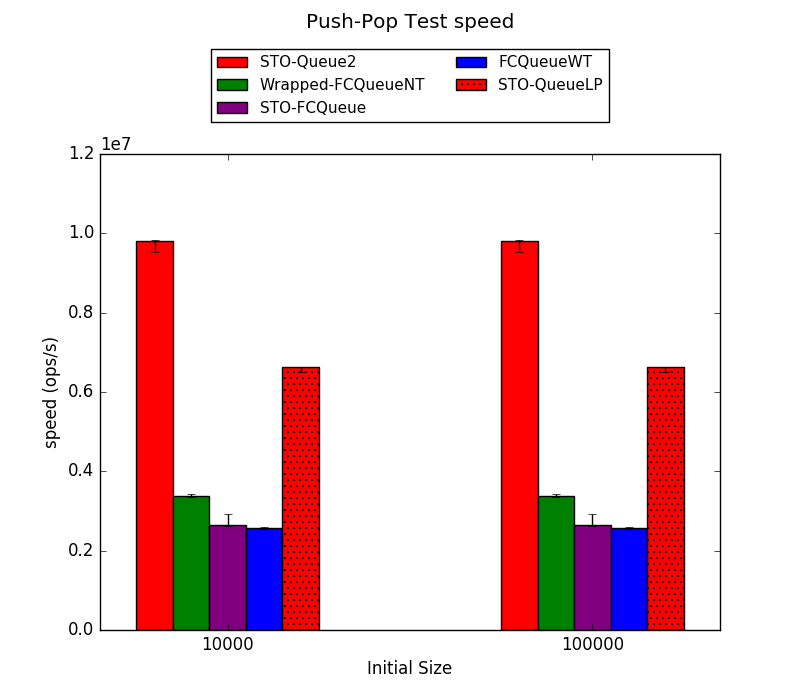
\includegraphics[height=2.25in]{fcqueues/lpQ:PushPopspeed.png} &
        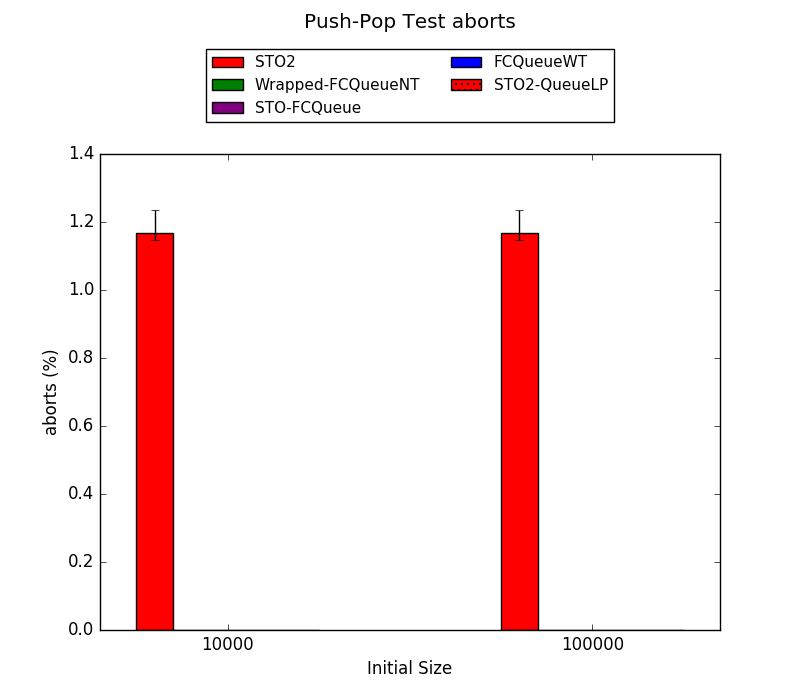
\includegraphics[height=2.25in]{fcqueues/lpQ:PushPopaborts.png}\\
        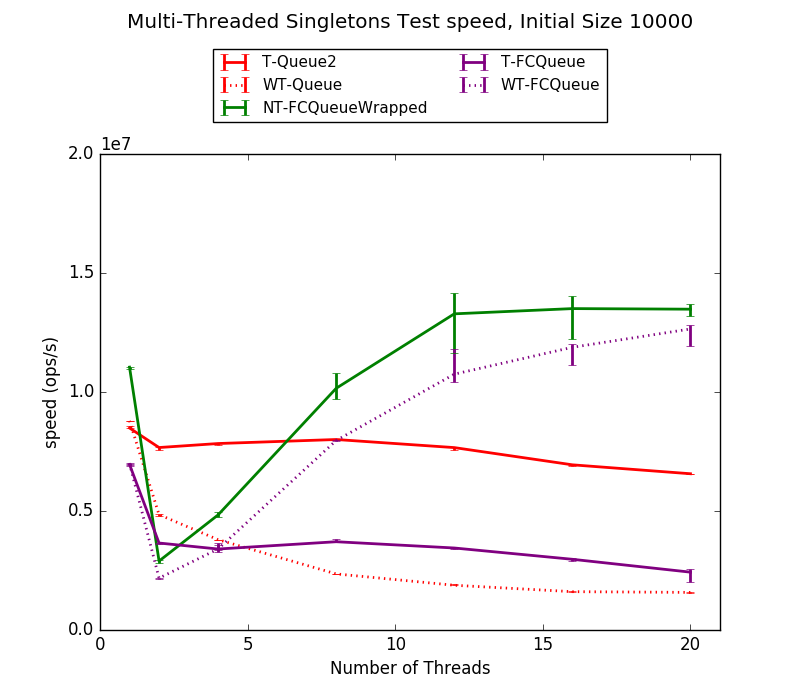
\includegraphics[height=2.25in]{fcqueues/lpQ:RandSingleOps10000speed.png} &
        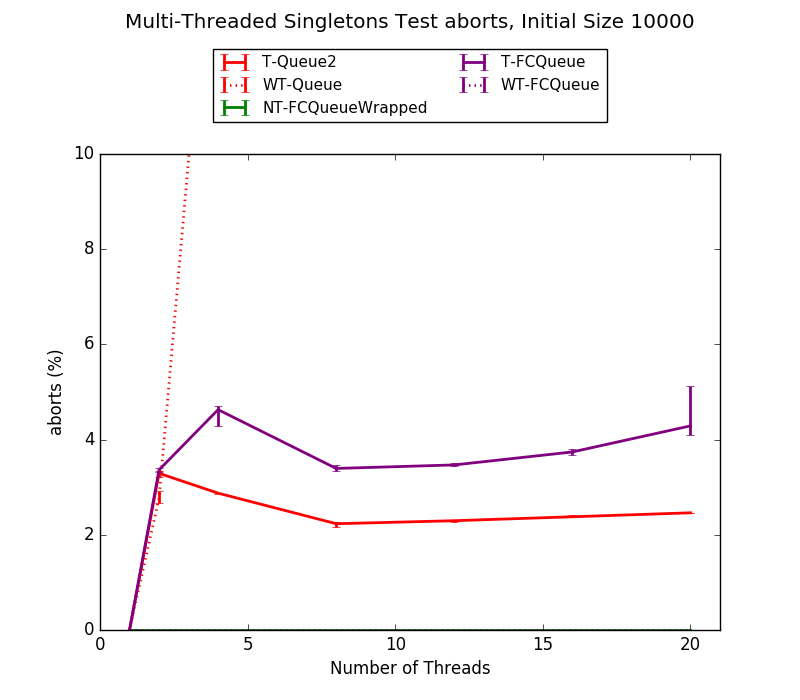
\includegraphics[height=2.25in]{fcqueues/lpQ:RandSingleOps10000aborts.png}\\
        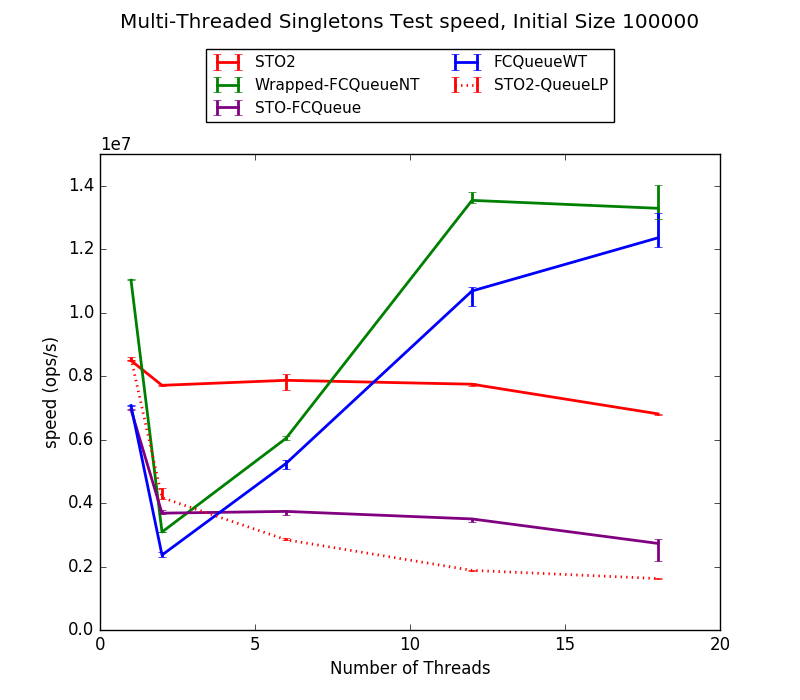
\includegraphics[height=2.25in]{fcqueues/lpQ:RandSingleOps100000speed.png} &
    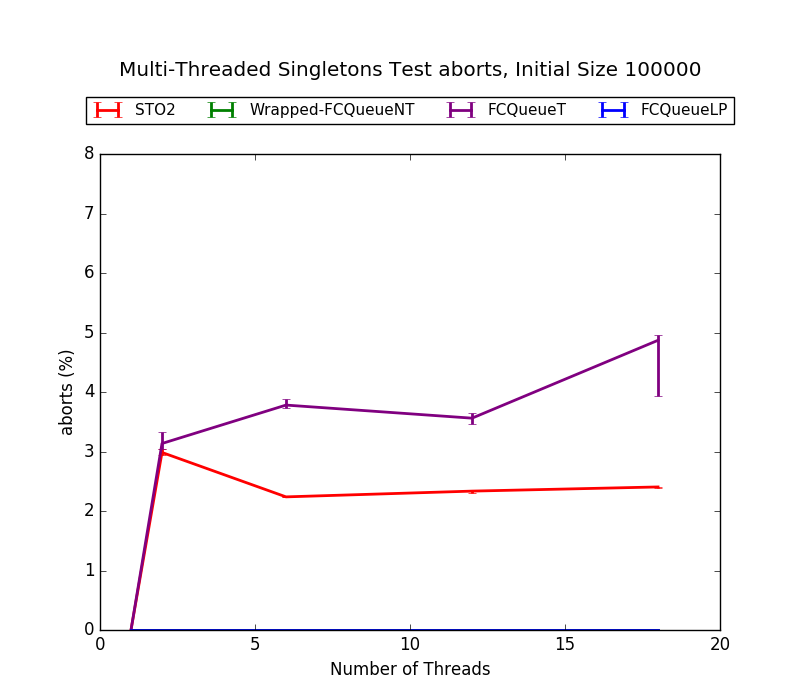
\includegraphics[height=2.25in]{fcqueues/lpQ:RandSingleOps100000aborts.png}\\
        \hline
    \end{tabular}
    \label{fig:lpfcqueues}
\end{figure}

While the weakly-transaction, flat combining queue (WT-FCQueue) does not perform as well as its nontransactional counterpart, NT-FCQueue, the performance of the WT-FCQueue exceeds that of the T-Queue1, the T-Queue2, and the T-FCQueue, which all provide full-transactional guarantees. We see gains in performance over the T-Queue2 up to 1.5$\times$ as the number of threads accessing the queue increases to 18; the WT-FCQueue begins to outperform the STO queue as the number of threads increases past 7. The WT-FCQueue outperforms the T-FCQueue starting at 4 threads and achieves performance up to about 3$\times$ by 18 threads.
 
The WT-FCQueue does not experience any aborts. This is due to the flat combining algorithm, which does not require that any locks be held in the weakly transactional setting in order to ensure correctness. A transaction can only abort if the result of a pop is accessed during the transaction's execution.

Because of the lack of aborts, the WT-FCQueue outperforms its counterpart, the WT-Queue; this demonstrates the effectiveness of the flat combining technique in the weakly transactional setting. The WT-Queue performs worse than all queues measured because of its high abort rate at commit time (100\% of aborts occur at commit time). This is caused by contention on the headversion and tailversion locks. While the actual pop function called during a transaction's execution is much simpler than in the T-Queue1 or T-Queue2 algorithms because it does not access the queue to check if the queue is empty, the installation procedure becomes more complicated because it requires instantiating all LazyPops, which also nearly triples the number of cache misses. The WT-FCQueue incurs approximately 1.5$\times$ more cache misses than the NT-FCQueue, but is not crippled from LazyPop-caused cache misses because the flat combining algorithm optimizes for efficient cache usage. Unlike the WT-FCQueue, the WT-Queue holds a global lock during installation at commit time, causing other transactions attempting to commit to abort.
